\section{Methodology}
\siyu{The current content of the ``Methodology'' section is too limited, try to expand this content.}

\figref{system_architecture} shows the architecture of the proposed system which takes as input multi-view color images of an object with known poses and outputs a triangle mesh of the object $ T = (V, F) $ where $ V = \{ v_i \in \mathbb{R}^3\} $ is the set of vertex coordinates and $ F \subseteq V \times V \times V $ is the set of faces.
The multi-view voxel grid prediction module (\subsecref{multiview_voxel}) first predicts a coarse voxel grid of the object.
The voxel grid is converted to mesh representation by \texttt{cubify} operation which is further refined by the mesh refinement module (\subsecref{mesh_refinement}).
A series of Graph Convolution Networks (GCN) deforms the cubified voxel grid to obtain surface mesh.
The GCNs use multi-view contrastive depth features from concatenated predicted and rendered depth along with RGB features as input to deform the input mesh.
Depth images are predicted using an extended MVSNet network~\cite{yao2018mvsnet}.
The multi-view features are fused using attention mechanism.

\siyu{Before Section 3.1, at least two point should be mentioned: 1. The input and output of this approach, including some notations. 2. An overview of the whole methodology including some reference of the explicit sections. And it is also a hierarchical structure of the ``Methodology'' section.}
\rakesh{updated the paragraph}

\subsection{Multi-view Voxel Grid Prediction}
\label{subsec:multiview_voxel}

\paragraph{Single-view Voxel Grid Prediction}
We adopt single-view voxel branch of~\cite{gkioxari2019meshrcnn} which consists of a ResNet feature extractor and a fully convolutional voxel grid prediction network. It generates the coarse initial shape of an object from one viewpoint as voxel occupancy grid using a color image. Here, we set the resolution of the generated voxel occupancy grid as 48 $\times$ 48 $\times$ 48. The voxel prediction networks for all viewpoints share the same weights.
% following Mesh R-CNN~\cite{gkioxari2019meshrcnn}.
\siyu{Should cite MeshRCNN reference here. As well, the implementation differences should be detailized here.}
\rakesh{cited Mesh RCNN, there are no implementation difference}

\paragraph{Probabilistic Occupancy Grid Merging}
\siyu{Present a figure to demonstrate the ``probabilistic occupancy grid merging'', the intermediate results of this module.}
\rakesh{The main system diagram shows the intermediate results, do we need another? I think we won't have enough space for it}

\siyu{This method is inspired by the traditional occupancy grid merging approaches in robotics? If so, try to cite the references and tell the differences between yours and the existed ones.}
\rakesh{citations added}

Voxel occupancy grid predicted from a single viewpoint suffers from occlusion and limited visibility.
In order to fuse voxel grids from different viewpoints we take inspiration from occupancy map building techniques in robotics~\cite{grisetti2007improved,konolige1997improved} and propose a probabilistic occupancy grid merging method which merges the voxel grids from each input viewpoint probabilistically to obtain the final voxel grid output.
This allows occluded regions in one view to be estimated from other views where those regions are visible as well as increase the confidence of prediction in overlapping regions.
Occupancy probability of each voxel is represented by $p(x)$ which is converted to log-odds (logit):
% \footnote{In practice the \emph{voxel branch} directly predicts the log-odds instead of probabilities}

\begin{equation}
    l(x) = log \frac{p(x)}{1 - p(x)}
    \label{equ:logodds}
\end{equation}

Bayesian update on the probabilities reduce to simple summation of log likelihoods~\cite{konolige1997improved}. Hence, the multi-view log-odds of a voxel is given by:

\begin{equation}
    l(x) = l_1(x) + l_2(x) + ... + l_n(x)
    \label{equ:logodds_sum}
\end{equation}

\noindent where $l_i$ is the voxel's log-odds in view $i$ and $n$ is the number of input views.
The final voxel probability $x$ is obtained by applying the inverse function of \equref{logodds} which is a sigmoid function.
% The final probability of the voxel $x$ can be obtained by applying the inverse function of \equref{logodds} which is a sigmoid function.

\siyu{We should add an experiment and study the effect of the quality of the initial mesh on the final mesh reconstruction results, including the ellipsoid, single-view MeshRCNN, our MeshRCNN with different number of views.}

\subsection{Mesh Refinement}
\label{subsec:mesh_refinement}
\siyu{Present a figure to explain the detailed mechanism of the mesh refinement module.}
\rakesh{I think the system architecture diagram and constrastive feature extraction diagram presents most of the details except graph convolution network and attention implementation. Do we want to show GCN and attention details in figures?}
The \texttt{cubified} mesh from the voxel branch only provides a coarse reconstruction of the object's surface. We apply graph convolutional networks which represent each mesh vertex as one graph node and deforms them to more accurate positions based on RGB and contrastive depth features.

\label{subsec:depth_prediction}
\paragraph{Multi-View Depth Estimation}
\siyu{In order to explain how can we obtain the initial depth images as the input, this paragraph should be put in front of the ``Mesh Refinement'' section, or the front of the ``3. Methodology''. We donot have to mention the details of MVS-Net, while some implementation details, like the view selection mechanism, resolution, network structure design, any difference from the standard MVS-Net or Cas-MVSNet.}
\rakesh{Paragraph moved to start of ``Mesh Refinement'' subsection. More details added}
We extend MVSNet~\cite{yao2018mvsnet} and predict the depth maps of all views since the original implementation predicts depth of only one reference view.
This is achieved by transforming the feature volumes to each view's coordinate frame using homography warping
and applying identical cost volume regularization and depth regression on each view.
Detailed network architecture diagram of this module is provided in the appendix.
Unlike~\cite{yao2018mvsnet}, we do not apply input image view selection and use the input views from~\cite{3dr2n2,wen2019pixel2mesh++} for fair comparison.
We set the number of depth hypothesis to $48$ which is equivalent to $25$ mm resolution.
\siyu{Do we have to add an experiment and compare the results give different settings of MVS-Net, such as the resolution of the depth images or we can add some noise to the depth. That is to study the effect of the quality of the depth on the final mesh reconstruction results and how sensitive is the refinement module to the depth quality.}

% which constructs a regularized 3D cost volumes
% to estimate the depth map of the reference view.
% Here, we extend MVSNet to predict the depth maps of all views instead of only the reference view.

% This allows the reuse of pre-regularization feature volumes for efficient multi-view depth prediction invariant to the order of input images.

\paragraph{GCN-based Mesh Deformation}
\siyu{The intuition and basic operations of graph-cnn-based mesh deformation should be given first. Then, how does the previous approach obtain the features. Any limitations and problems of the previous approaches?}

A graph convolution deforms mesh vertices by propagating features from neighboring vertices by applying
$f_{i}^{'} = ReLU(W_0f_i + \sum_{j \in \mathcal{N}(i)} W_1 f_j)$ where $\mathcal{N}(i)$ is the set of neighboring vertices of the \emph{i}-th vertex in the mesh, $f_{\{\}}$ represents the feature vector of a vertex, and $W_0$ and $W_1$ are learnable parameters of the model.
The features pooled from multi-view images (discussed in subsequent paragraphs) along with 3D coordinates of the vertices in world frame are used as features of the graph nodes.
Series of Graph-based Convolutional Network (GCN) blocks are applied to deform a mesh at the current stage to the next stage, starting with the \texttt{cubified} voxel grids.
Each GCN block utilizes several graph convolutions to transform the vertex features along with a final \emph{vertex refinement} operation where the features along with vertex coordinates are further transformed as $v_i^{'} = v_i + tanh(W_{vert}[f_i;v_i])$ where the matrix $W_{vert}$ is another learnable parameter to obtain the deformed mesh.

\label{subsec:contrastive_depth_feature_extraction}
\paragraph{Contrastive Depth Feature Extraction}

\siyu{Can you give a figure demonstrating the module of contrastive depth feature extraction? Since in Figure 1 of the ICLR submitted paper, you also input the RGBD feature maps from ResNet, do you still use it?}
\rakesh{Figure added. RGBD features are still used and the new system diagram also shows it}

\begin{figure}[h!]
    \begin{center}
        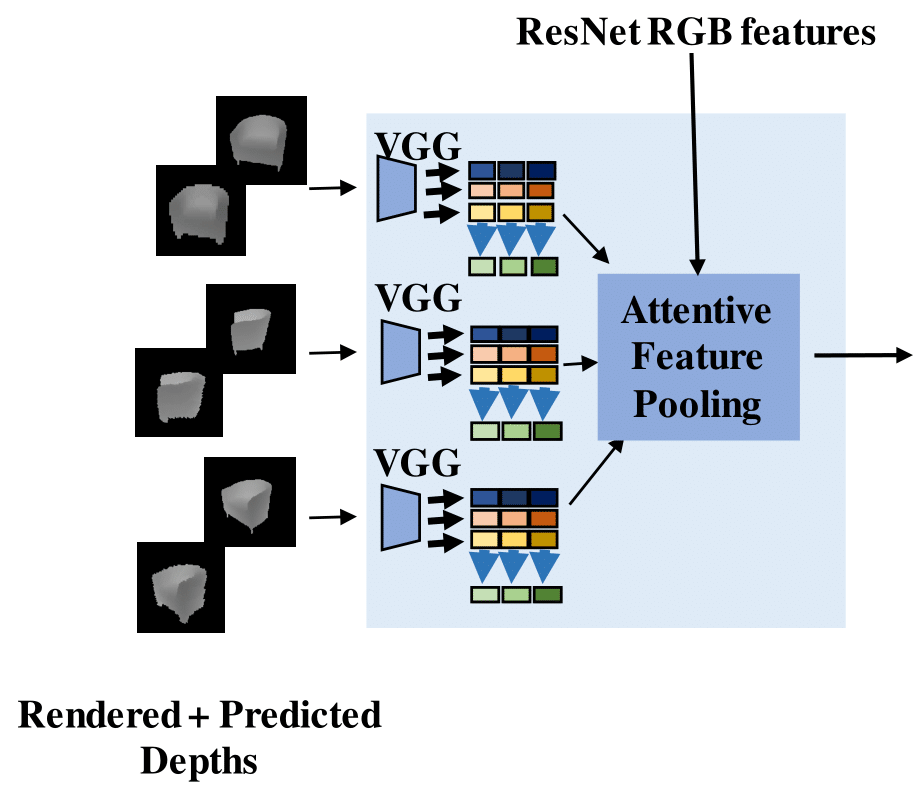
\includegraphics[width=\linewidth]{imgs/contrastive_feature_extractor.png}
    \end{center}
    \vspace{-4mm}
        \caption{Contrastive feature extraction. Rendered depths of the current shape along with the predicted depths for each view are concatenated and VGG-based feature extractor is applied. The multi-view features are pooled using attentive feature pooling and used by GCN for deforming the shape}
        \vspace{-4mm}
        \label{fig:contrastive_feature_extractor}
\end{figure}

\cite{yao2020front2back} demonstrate that using intermediate, image-centric 2.5D representations instead of directly generating 3D shapes in global frame from raw 2D images can improve 3D reconstruction quality.
We therefore propose to formulate the features for graph nodes using 2.5D depth maps as input additional inputs alongside the RGB features.
% and \zhiwen{todo} to contrast the depth map at current refinement stage against the predicted depths.
Specifically, we render the meshes at different GCN stages to depth image at all the input views using~\cite{kato2018renderer} and use them along with predicted depths for depth feature extraction. We call this form of depth input \texttt{contrastive depth} as it contrasts the rendered depths of the current mesh against the predicted depths and allows the network to reason about the deformation better than when using predicted depth or color images alone.
% construct the feature vector from semantic features of the input color images~\cite{wang2018pixel2mesh}, we formulate the input for feature extraction network using geometry representations.
% However, works similar to Pixel2Mesh~\cite{wang2018pixel2mesh} construct the feature vector from semantic features of the input color images. Here, we formulate the input for feature extraction network using geometry representations. Specifically, we render the meshes at different GCN stages to depth image at all the input views using~\cite{kato2018renderer} and augment them as additional inputs for depth feature extraction.
% We call this form of depth input \emph{contrastive depth} as it contrasts the rendered depths of the current mesh against the predicted depths and constrain the deformed mesh in a coarse-to-fine manner.
Given the 2D features, corresponding feature vectors of individual vertices can be found by projecting the 3D vertex coordinates to the feature planes using known camera parameters.
We use VGG-16~\cite{simonyan2014vgg} as our contrastive depth feature extraction network.
% Along with the contrastive depth features, we also use the RGB features from ResNet calculated for voxel branch as input for mesh deformation as well.

% and allows the network to reason about the deformation required better than when using predicted depths alone.
% Multiple methods for augmenting the two depths were tried among which using concatenated rendered and predicted depth as input for depth feature extraction gave the best result.
% Along with the contrastive depth features, we also use the RGB features from ResNet calculated for voxel branch as input for mesh deformation as well.

\begin{figure*}[t]
\begin{center}
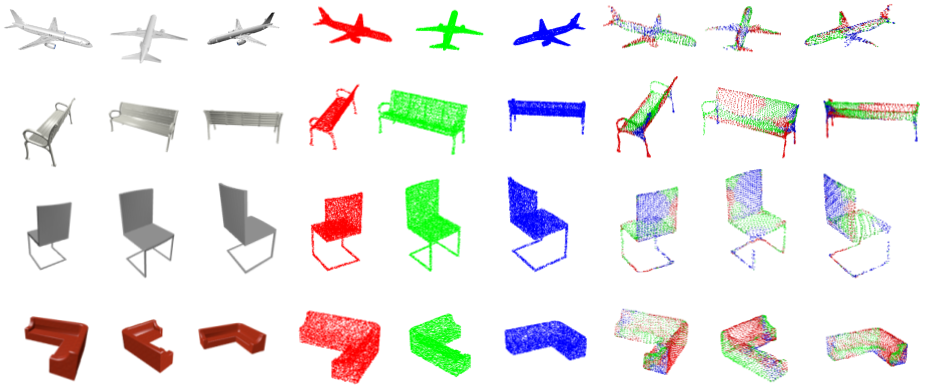
\includegraphics[width=\linewidth]{imgs/attention_weights_visualization.png}
\end{center}
    \caption{
        \textbf{Attention weights visualization.}
        From left to right: input images from 3 viewpoints, corresponding ground truth point clouds color-coded by their view order and the predicted mesh vertices color-coded by the attention weights of the views.
        Only the view with maximum attention weight is visualized for each predicted points for clarity.
    }
\label{fig:attention_weights}
\end{figure*}

\paragraph{Attention-based Multi-View Feature Pooling}
In order to fuse multi-view contrastive depth features, we formulate an attention module by adapting multi-head attention mechanism originally designed for sequence to sequence machine translation using transformer (encoder-decoder) architecture~\cite{vaswani2017attention}.
% \rakesh{Transformer architecture was proposed in multi-head attention paper, it doesn't need a separate citation}
In a transformer architecture the encoder hidden state is mapped to lower dimension key-value pairs (\textbf{K}, \textbf{V})
while the decoder hidden state is mapped to a query vector \textbf{Q} using independent fully connected layers.
The encoder hidden state in our case is the multi-view features while the decoder hidden state is the \emph{mean} of the multi-view features.
The attention weights are computed using scaled-dot product:
\begin{equation}
    Attention(\mathbf{Q}, \mathbf{K}, \mathbf{V}) = softmax(\frac{\mathbf{Q} \mathbf{K}^{T}}{\sqrt{N}}) \mathbf{V}
    \label{equ:attention}
\end{equation}
\noindent where $N$ is the number of input views.

Multiple attention \emph{heads} are used which are concatenated and transformed to obtain the final output
\begin{align}
    head_i = Attention(\mathbf{Q} \mathbf{W}^{Q}_{i}, \mathbf{K} \mathbf{W}^{K}_{i}, \mathbf{V} \mathbf{W}^{V}_{i}) \label{equ:attention_head} \\
    MultiHead(\mathbf{Q}, \mathbf{K}, \mathbf{V}) = [head_1; ...; head_h] \mathbf{W}^0 \label{equ:multihead_attention}
\end{align}

\noindent where multiple $\mathbf{W}$ are parameters to be learned,
$h$ is the number of attention heads and $i\in[1,h]$.

% We refer our readers to~\cite{vaswani2017attention} for further technical details.

We choose multi-head attention as our feature pooling method since it allows the model to attend information from different representation subspaces of the features by training multiple attentions in parallel.
This method is also invariant to the order and number of input views.
We visualize the learned attention weights (average of each attention heads) in~\figref{attention_weights} where we can observe that the attention weights roughly takes into account the visibility/occlusion information from each view.
% instead of other forms of attention (e.g.~\cite{chorowski2015attention,luong2015effective}) because


% The network architectures of the GCN blocks are identical to Mesh R-CNN's implementation.
% We refer readers to~\cite{wang2018pixel2mesh,gkioxari2019meshrcnn} for further details.

% \rakesh{Differentiable Depth Rendering is just "Neural Renderer" without any change. This has already been covered in system overview}
% \subsection{Differentiable Depth Rendering}
% In order to add constrains of all intermediate predicted meshes, previous mesh generation methods~\cite{wang2018pixel2mesh} add loss terms to prevent the meshes deform too much. Here, we refer Neural Renderer~\cite{kato2018renderer} to differentiably render predicted meshes to depth images at all the input views.
% It approximates the gradients for rendering a mesh enabling back-propagation of losses defined on the rendered depths.
% % More recently methods that render depth without approximating the gradients have been proposed~\cite{liu2019soft};
% % but since it does not support depth rendering we use Neural Renderer.
% Note that any differentiable depth renderer can be used in its place.
%
% Prior works~\cite{kato2018renderer,liu2019soft} have used differentiable renderers in order to reconstruct 3D objects.
% These work rely solely on the rendered images or silhouettes for reconstruction.
% Since we directly supervise on 3D models during training, we use the rendered depths only for regularization.
% Specifically, the difference between the rendered depths and predicted depths at corresponding viewpoints are used as loss terms.
% The exact loss functions are described in \subsecref{losses}.

\subsection{Loss functions}
\label{subsec:losses}
% For training the mesh generation, we use the loss terms from~\cite{wang2018pixel2mesh} along with new losses based on our formulation.

\paragraph{Mesh losses}
The losses which are derived from~\cite{wang2018pixel2mesh} to constrain the mesh predicted by each GCN block (P) to resemble the ground truth (Q) include
Chamfer distance $\mathcal{L}_{\text{chamfer}}(\text{P}, \text{Q}) = |\text{\text{P}}|^{-1} \sum_{(p, q) \in \Lambda_{\text{P},\text{Q}}}{||p-q||^{2}} + |\text{Q}|^{-1} \sum_{(q, p) \in \Lambda_{\text{Q},\text{P}}}{||q-p||^{2}}$
and surface normal loss
$\mathcal{L}_{\text{normal}}(\text{P}, \text{Q}) = -|\text{P}|^{-1} \sum_{(p, q) \in \Lambda_{\text{P},\text{Q}}}{|u_p \cdot u_q|} - |\text{Q}|^{-1} \sum_{(q, p) \in \Lambda_{\text{Q},\text{P}}}{|u_q \cdot u_p|}$
with additional regularization in the form of edge length loss
$\mathcal{L}_{\text{edge}}(\text{V}, \text{E}) = \frac{1}{|E|} \sum_{(v,v') \in E}{||v - v'||^2}$
for visually appealing results.
% \cite{wen2019pixel2mesh++} report improved performance when using Chamfer distance loss where the predicted mesh is re-sampled to obtain a point cloud with larger number of points.
% We do not observe such improvements (the performance is even worse).
% Note that~\cite{wen2019pixel2mesh++} uses mesh generated by Pixel2Mesh~\cite{wang2018pixel2mesh} as input and further refines it while our predictions are obtained without such initialization which might explain this difference.
% Nonetheless, for evaluation we use re-sampled Chamfer distance for a fair comparison.

\paragraph{Depth loss}
Our depth prediction network is supervised using adaptive reversed Huber loss (also known as BerHu criterion)~\cite{lambert2016adaptiveberhu}.
% This loss has been used for depth prediction in previous work such as~\cite{tang2018ba,laina2016deeper}.
$\mathcal{L}_{depth} = |x|, & \text{if}\ |x| \le c \text{, otherwise } \frac{x^2 + c^2}{2c}$ where $x$ is the depth error of a pixel and $c$ is a constant set to $0.2$.
Note that the original MVSNet uses L1-loss, but we used BerHu loss since it gave slightly higher accuracy.
Intuitively, this is because BerHu provides a good balance between L1 and L2 loss and has shown similar improvement in~\cite{laina2016deeper}.

\paragraph{Contrastive depth loss}
% Additional loss terms for mesh generation supervision can be derived from the available depth predictions at different views to add extra constraints on the generated mesh, providing a form of self-supervision.
% The meshes predicted by different GCN blocks are differentiably rendered from the viewpoints of the predicted depth images and
BerHu loss is also applied between the rendered depth images at different GCN stages and the predicted depth images.
% which encourages the predicted mesh to conform to the predicted depths.
$\mathcal{L}_{contrastive} = |x|, & \text{if}\ |x| \le c \text{, otherwise } \frac{x^2 + c^2}{2c}$

\paragraph{Voxel loss} Binary cross-entropy loss between the predicted voxel occupancy probabilities and the ground truth occupancies is used as voxel loss to supervise the voxel predictions
% Voxel loss is introduced for the final probabilistically merged voxel grid as well as the voxel grids of individual views.
$\mathcal{L}_{\text{voxel}} = -{\Big(p(x) log\big(p(x)\big) + \big(1 - p(x)\big)log\big(1 - p(x)\big)\Big)}$

\paragraph{Final loss} We use the weighted sum of the individual losses discussed above as the final loss to train our model in an end-to-end fashion.
$\mathcal{L} = \lambda_{\text{chamfer}}\mathcal{L}_{\text{chamfer}} + \lambda_{\text{normal}}\mathcal{L}_{\text{normal}} + \lambda_{\text{edge}}\mathcal{L}_{\text{edge}} + \lambda_{\text{depth}}\mathcal{L}_{\text{depth}} + \lambda_{\text{contrastive}}\mathcal{L}_{\text{contrastive}} + \lambda_{\text{voxel}}\mathcal{L}_{\text{voxel}}$
, where $\mathcal{L}$ is the final loss term.

\siyu{We should discuss each loss function in more details. In addition, the description of $\mathcal{L}_{\text{chamfer}}$, $\mathcal{L}_{\text{normal}}$ and $\mathcal{L}_{\text{edge}}$ should be discussed in more details, including the intuition and functionality.}
